\documentclass[border=10pt]{standalone}
%%%<
\usepackage{verbatim}
%%%>
\usepackage{pgfplots}
\pgfplotsset{width=7cm,compat=1.8}
\usepackage{pgfplotstable}
\begin{comment}
:Title: Plotting several 2d functions in a 3d graph
:Tags: 2D;3D;Functions;Mathematics
:Author: Jake
:Slug: 2d-functions-in-3d

We would like to plot several two-dimensional functions in a
three-dimensional graph.

Tabulated data can be plotted in different planes quite easily by using
\addplot3 table [y expr=<value>, z=<name of column in table>]
{<file name or table macro>};.

We can use \pgfplotsinvokeforeach{<list expression>}{...} to repeat the
plot commands. Here's an example of how to plot some dummy data.

A second example shows plotting a couple of math functions.
This code was written by Jake on TeX.SE.
\end{comment}
\begin{document}
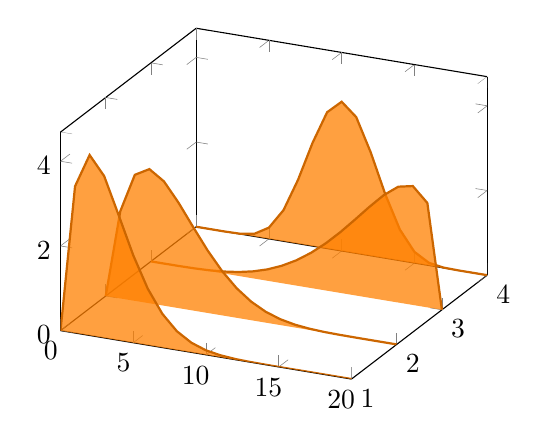
\begin{tikzpicture}

\pgfplotstableread{
plot1   plot2   plot3   plot4
0       0       0       0
3.466   2.058   0       0
4.262   2.976   0.001   0
3.822   3.168   0.006   0.008
2.953   2.936   0.019   0.063
2.065   2.492   0.046   0.265
1.332   1.977   0.092   0.734
0.797   1.478   0.164   1.508
0.443   1.045   0.268   2.44
0.228   0.698   0.412   3.219
0.107   0.438   0.598   3.524
0.046   0.256   0.831   3.219
0.017   0.138   1.109   2.44
0.006   0.067   1.429   1.508
0.002   0.029   1.78    0.734
0       0.01    2.141   0.265
0       0.003   2.479   0.063
0       0.001   2.736   0.008
0       0       2.808   0
0       0       2.465   0
0       0       0       0
}\dummydata
\begin{axis}[
    samples=30,
    domain=-4:4,
    samples y=0, ytick={1,...,4},
    zmin=0,
    area plot/.style={
        fill opacity=0.75,
        draw=orange!80!black,thick,
        fill=orange,
        mark=none,
    }
]
\pgfplotsinvokeforeach{4,3,...,1}{
    \addplot3 [area plot] table [x expr=\coordindex, y expr=#1, z=plot#1]
      {\dummydata};
}
\end{axis}
\end{tikzpicture}
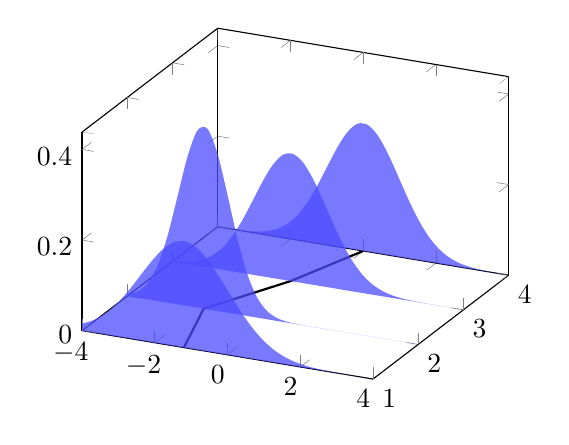
\begin{tikzpicture}[
    declare function={
        normal(\m,\s)=1/(2*\s*sqrt(pi))*exp(-(x-\m)^2/(2*\s^2));
    }
]
\begin{axis}[
    samples=30,
    domain=-4:4,
    samples y=0, ytick=data,
    zmin=0,
    area plot/.style={
        fill opacity=0.75,
        draw=none,
        fill=blue!70,
        mark=none,
        smooth
    }
]
\addplot3 [black, thick] table {
0 4 0
-0.75 3 0
-1.9 2 0
-1.2 1 0
};
\addplot3 [area plot] (x,4,{normal(0,1)});
\addplot3 [area plot] (x,3,{normal(-0.75,1)}) -- (axis cs:-4,3,0);
\addplot3 [area plot] (x,2,{normal(-1.9,0.7)}) -- (axis cs:-4,2,0);
\addplot3 [area plot] (x,1,{normal(-1.2,1.2)}) -- (axis cs:-4,1,0);
\end{axis}
\end{tikzpicture}
\end{document}